\section{Overview}

Static binary instrumentation is a process that leaves a modified executable on
disk that can be run at a later time. Then when the instrumented executable is
run, the extra instrumentation code inserted by the instrumentation tool is run
in addition to the normal behavior of the program. In order to insert extra code
and data, extra space must be allocated within the executable in a way that it
will, at load-time, be treated by the system in a manner appropriate to its
purpose. Consider the following. Most compilers emit an executable whose
structure is similar to that shown in Figure \ref{Figure:Executable}. By
convention, most executables use only two loadable segments and certain Linux
implementations such as FreeBSD only allow two loadable segments. Thus it is
preferrable for us to incorparate instrumentation text and data into the
existing text and data segments of the application. The default in most
compilers is to place the text segment prior and adjacent to the data segment.
We therefore prepend the instrumentation text to the existing text
segment\footnote{The amount of space allocated prior to the text section is
controlled by the linker variable \_\_executable\_start. We have seen cases
where the system does not provide enough space prior to the text segment by
default, in which case we provide a set of tools that produces a modified linker
script that provides 128Mb of space.} and append the instrumentation data to the
data segment, which can be seen in Figure \ref{Figure:InstExecutable}. This
scheme has the added benefit of causing no immediate disturbance to the
addresses of the existing text and data segments of the program.

\begin{figure}[ht]
\centering
\caption[Optional caption for list of figures]{\subref{Figure:OrigExecutable} and \subref{Figure:InstExecutable} show the prepending
of instrumentation text to the existing text, and the prepending of instrumentation data to the existing data respectively.}
\subfigure[The two-segment structure of an unmodified ELF file.]{
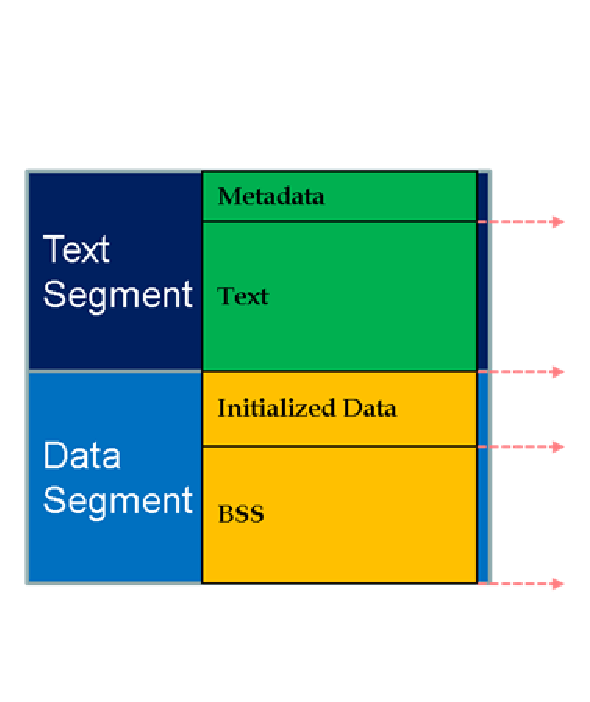
\includegraphics[scale=0.65]{executablep1.eps}
\label{Figure:OrigExecutable}
}
\subfigure[The two-segment structure of the ELF file once instrumentation code and data are inserted.]{
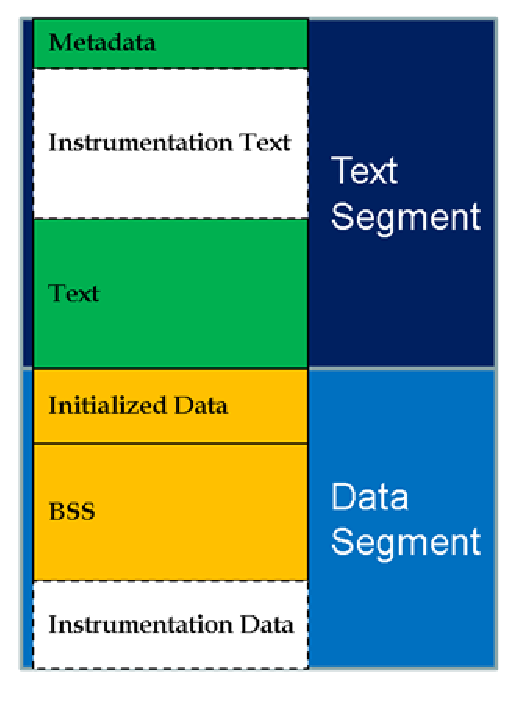
\includegraphics[scale=0.65]{executablep2.eps}
\label{Figure:InstExecutable}
}
\label{Figure:Executable}
\end{figure}

The instrumentation text contains several code of several kinds. The first
contains code that accomplishes the instrumentation task as well as some code to
accompany it. When control is transferred from the application to the
instrumentation code, it is necessary to maintain the pristine machine state of
the application in order to preserve its original behavior. This machine state
can contain anything modified by the instrumentation code, but in practice is
usually limited to a relatively limited set of registers. The trampoline will
save any registers it intends to use, perform the instrumentation task, restore
any machine state after the instrumentation task is complete, execute the
applications instructions that were displaced by the initial control transfer,
finally restoring control to the application. Since we are using an
unconditional branch instruction at the instrumentation point, at runtime the
instrumentation code has no information about where control was transferred from
(as might be the case if we used a more heaviweight call instruction). Hence
each instrumentation point uses its own trampoline so that the location of the
instrumentation point can be hard-coded into an unconditional branch instruction
at the end of the trampoline.

The instrumentation text also includes code to initialize data for use by the
instrumentation tool. Recall from Figure \ref{Figure:Executable} that the instrumentation
data was appended to the end of the application's data segment, after the
application's bss (uninitialized data) section. The initialized data and bss
sections of the data segment are usually implemented by declaring the size of
the data segment in the executable to be smaller than the size of the data
segment in memory. According to the ELF specification, the extra part of any
segment whose memory size is greater than its file size should be filled with
zeroes by the loader. Hence most programs just increase the size of the data
segment's size in memory by the size of the bss section in order to get a large
area that is filled with zeroes and is reserved for uninitialized data. Since we
would like to use the area following the bss section for (possibly initialized)
data for the instrumentation tool, we can either explicitly include the entire
segment's contents in the executable file or we can implicitly reserve this area
using the technique described above that is already in use by most programs.
Since the bss section can be very large and explicit inclusion of its contents
would bloat the instrumented executable file unnecessarily, we use the implicit
technique to reserve this section for instrumentatoin data. We therefore
temporarily store the instrumentation data with the instrumentation text in the
executable, as well as some code to copy it to the appropriate location in the
data segment once the program starts.
